%!TEX root = ../template.tex
%%%%%%%%%%%%%%%%%%%%%%%%%%%%%%%%%%%%%%%%%%%%%%%%%%%%%%%%%%%%%%%%%%%%
%% chapter3.tex
%% NOVA thesis document file
%%
%% Chapter with iCBD project
%%%%%%%%%%%%%%%%%%%%%%%%%%%%%%%%%%%%%%%%%%%%%%%%%%%%%%%%%%%%%%%%%%%%


%%-------------------------------------------------------------------
%%	3 - iCBD - Infrastructure for Client-Based (Virtual) Desktop (Computing)
%%-------------------------------------------------------------------
\chapter{iCBD - Infrastructure for Client-Based Desktop}
\label{cha:icbd}

The acronym \gls{iCBD} stands for Infrastructure for Client-Based (Virtual) Desktop (Computing). Is a platform being developed by an R\&D partnership between \textit{NOVA LINCS}, the Computer Science research unit hosted at the \textit{Departamento de Informática of Faculdade de Ciências e Tecnologia of Universidade NOVA de Lisboa} (DI-FCT NOVA) and \textit{SolidNetworks – Business Consulting, LDA} part of the \textit{Reditus S.A.} group. 

Where the primary goal is to achieve a particular kind of \gls{VDI} infrastructure, a client based VDI, where client's computations are performed directly on the client hardware as opposed to on big and expensive servers. With the distinctive characteristic of not having the necessity of investing in hard disks for the client devices, as well as hoping to solve prominent predicaments in the administration and management of large-scale computer infrastructure.

This chapter will address the central concepts and associated technologies encompassed in this project, particularly:\\

\begin{description}
	%
	\item [Section~\ref{sec:icbd_concept}] overviews the core concepts of the project and particularly note the limitations and peculiarities of current implementations in contrast with the chosen approach.
	%
	\item [Section~\ref{sec:icbd_architecture}] studies the principal architectural components of the platform, with emphasis on the different layers and how  they act together to serve the end-user.
	%
	\item [Section~\ref{sec:replication_cache}] will at last state the problem and motivation for introduction replication techniques in the storage components of the platform. Moreover, the section prefaces the importance of the implementation of cache servers that hold part of the distribution burden and crucial for the support of an increased number of clients.
\end{description}


%%-------------------------------------------------------------------
%%	3.1 - The Concept
%%-------------------------------------------------------------------
\section{The Concept} % (fold)
\label{sec:icbd_concept}

The iCBD as a project pretends to investigate and develop an architecture that leads to the birth of a platform that can operate desktop virtualisation (\gls{VDI}). In a sense, the goal is similar to a client-based VDI, but with the distinction of maintaining all the benefits of both client-based and server-based VDI. Additionally, it should present the power of working as a Cloud \gls{DaaS} without any of the bad traits of the approaches as mentioned earlier.

The aim is to preserve the convenience and simplicity of a fully centralised management platform for Linux and Windows desktops, instantiating those in each physical workstation from virtual machine templates (VMs) kept in repositories. We will talk more about this subject in section \ref{sec:icbd_architecture}\\

To summarise the platform should be able to:

\begin{itemize}
	\item Tuning to a wide range of server configurations, without prejudice to the defined architecture.
	%
	\item Minimize disruption in the use of workstations for end-users. Offering a work environment and experience of use so close to the traditional one that they should not be able to tell from a standard local installation of an \gls{OS} to the use of this platform.
	%
	\item Simplify installation, maintenance and platform management tasks for the entire infrastructure, including servers in their multiple roles, storage and network devices from a single point.
	%
	\item Allow for a highly competitive per workstation cost.
	%
	\item Maintain an inter-site solution; such a geographically disperse multi-office structure.
\end{itemize}


%%-------------------------------------------------------------------
%%	3.2 - The Architecture 
%%-------------------------------------------------------------------
\section{The Architecture} % (fold)
\label{sec:icbd_architecture}

%Topics:
%Introduce the layers
%Draw a diagram 
%Layers are a kind of role, not a single a defined service but a collection 

The iCBD platform comprehends the use of multiple services that take responsibility for an essential set of tasks. To achieve a better understatement of the inner workings of the system we can group these services in four major architectural labels as seen in the figure~\ref{fig:icbd_layers}.


\begin{figure}[htbp]
	\centering
	
\includegraphics[height=4in]{placeholder}
	\caption{iCBD Layers View}
	\label{fig:icbd_layers}
\end{figure}


\begin{description}
	\item [\acrfull{iMI}] a nomenclature borrowed and adapted from Amazon Web Services AMI~\cite{aws_ami} embodies the required files to run a iCBD platform client. Including a VM template (with an operating system, configurations and applications) the iCBD boot package ( a collection of files needed for a network boot and custom-made to the operating system) and an assortment of configurations for services like PXE and iSCSI.
	%
	\item [Boot Services Layer] is responsible for providing the initial process from which the client machines will boot from the network and the posterior transference of a bespoke boot package. Employing services such as \acrshort{PXE}, \acrshort{DHCP}, \acrshort{TFTP} and \acrshort{HTTP}.
	%
	\item [Administration Layer] (in regards to software) takes advantage of a virtualisation stack (can be based in either \acrshort{KVM} or VMWare products) to engage in maintaining all the needed aspects for the successful creation and update processes of an \acrshort{iMI} lifecycle.  Employing a custom set of scripts, the creation of an iCBD Boot Package is also a duty of this layer. 
	%
	\item [Client Support Layer] deals with the demands of a deployed and running iCBD image, such as, providing read/write space (since iMIs run on diskless workstations) and storing users home directories. As well as, hosting domain controllers, centralised authentication amongst other services that can be already in place in the midst of a clients infrastructure. Granting the ability to deploy a customised iMI in any scenario.
	%
	\item [Storage Layer] is accountable for maintaining the repository of iMIs and facilitate essential operations like version controlling the VM images files. Is also in this layer that we seize the potential of replication features provided by the file systems employed. In this project, the storage relies on two mainstream file systems: BTRFS and CEPH. Together with services like \acrshort{NFS} and \acrshort{iSCSI} enables a way to export data to clients.
\end{description}
 
Let's view in more detail each one of them.

%%-------------------------------------------------------------------
%%	3.2. - iCBD Machine Image 
%%-------------------------------------------------------------------
\subsection{iCBD Machine Image}
\label{sub:icbd_architecture_imi}

\begin{figure}[htbp]
	\centering
	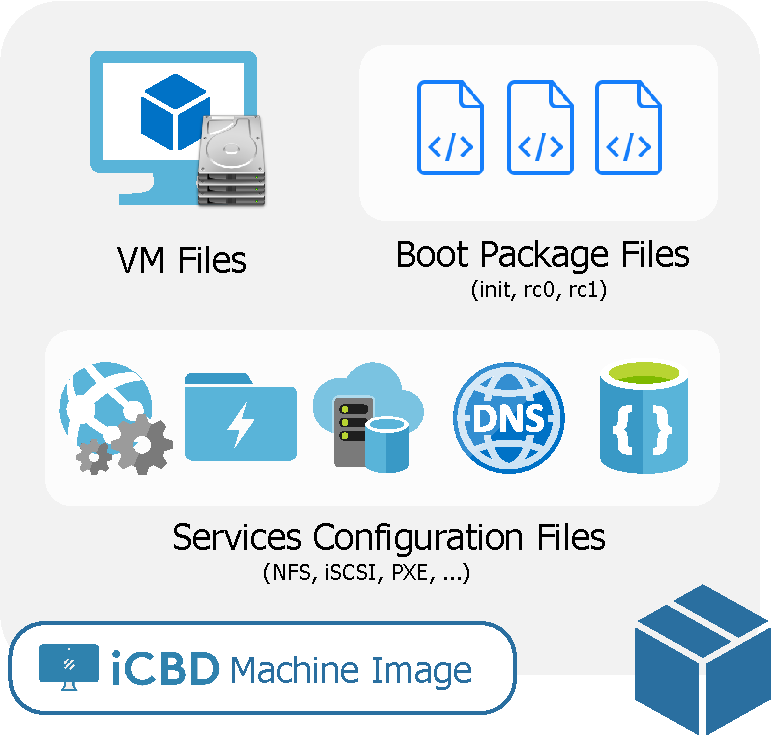
\includegraphics[height=4in]{cap3_iMI}
	\caption{iCBD Machine Image Files}
	\label{fig:icbd_iMI_files}
\end{figure}

In its essence, an iCBD Machine Image is the compilation of everything that is needed to run an Operating System within the iCBD platform, that is data and configuration files. For the sake of simplicity, we may categorise the files in three main groups.

\begin{description}
	\item [VM Template files] The main component is the virtual machine template in the form of a read-only image. As described in section~\ref{sub:vm_storage} the anatomy of a template follows the standard from VMware and KVM VMs either with multiple files (i.e., Virtual Disk Files like \texttt{.vmdk} or \texttt{.qcow}) or a \textit{RAW} storage format.
	%
	\item [iCBD Boot Package files] In a network boot environment, as the one used, there is a need to keep a set of files that manage the boot of a workstation; these can be included in the initial \textit{ramdisk} or later transferred over HTTP when needed. Included are an init file and at least two Run Control Script files (\texttt{rc0} and \texttt{rc1}) that are responsible for starting network services, mounts all file systems and ultimately bring the system up in single-user level. With a tool such as \textit{BusyBox} (a single executable file with a stripped-down set of tools), a basic \textit{shell} is available during the boot process to fulfil all the required configurations.
	%
	\item [Services Configuration files] Among the services employed there is the need for changes in some of the configurations files of these services. The NFS exports configuration file should reflect a structure of which file systems are exported, the networks that a remote host can use, as well as, a myriad of options that the NFS allows to be set. The same happens to iSCSI where an iSCSI targets need to refer to a backing store of the storage resource where the image resides. 
\end{description}



%%-------------------------------------------------------------------
%%	3.2. - Boot Layer 
%%-------------------------------------------------------------------
\subsection{Boot Services Layer}
\label{sub:icbd_architecture_boot}
% https://opensource.com/article/18/1/analyzing-linux-boot-process
% https://www.ibm.com/developerworks/library/l-linuxboot/index.html
% https://utcc.utoronto.ca/~cks/space/blog/linux/LinuxBootOverview?


From an end-user perspective, the only layer that is visible and interactive is the boot layer. The interface is lean and provides a way to select the image to boot in the workstation, however not every single aspect is noticeable. In the background, there is a need to resort to multiple services for starting a client's workstation with an iCBD Machine Image.

The platform provides two processes to remote boot an iMI. One instantiates, from an iMI, the Operating System natively on the bare metal workstation in the fashion of a standard diskless network boot. The other uses the above mechanism for provisioning a minimal iMI that was a hypervisor installed and virtualises any other iMI available in the storage layer. Both approaches are entirely transparent to the final user that does not grasp the differences and doesn't know if the working OS is virtualised or running natively.

The first part of the boot process starts like any other network boot, where a series of DHCP requests are used to provide the suitable client network parameters and particularly the location (IP address) of the TFTP server. Then begins the transference of a small network boot manager program. In this traditional PXE boot environment, a friendly looking tailored made graphical menu displays to the user an assortment of choices that announce the different iMIs ready to boot.

\subsubsection{Booting an iMI}
\label{susub:booting_imi}
%(REF https://www.ibm.com/developerworks/library/l-initrd/index.html)
After the selection of an iMI in the PXE boot menu~\cite{ibm_linux_boot} the second-stage boot kicks in. Using \textit{PXELINUX} as a bootloader there is the capability of transferring a compressed Linux Kernal (vmlinuz) and an initial ramdisk (initrd) (REF in comment)through either TFTP or HTTP, is also in this step that some parameters needed during the boot are set with the correct values according to the image picked. After everything loaded into memory, the stage 2 boot loader invokes the kernel image, and after booted and initialised, the kernel starts the first user-space application. 

Commonly the first application is called init, and in the particular case of this platform, the init file starts the chain execution of other custom files (\texttt{rc0} and \texttt{rc1}). Those Run Control scripts configure every single aspect in the Operating System according to the characteristics of physical machine booting. The first step is to reconfigure the network card and obtain connectivity. Then, is determined if there is the need for getting more files indispensable for the remaining boot process if this need exists, then the missing files are transferred. The next script, \texttt{rc0}, deals with data volumes and their mounting method (i.e. r/w space, users home directories); in case of using the loading OS as a base for another iMI in virtualisation, some configurations are anticipated and applied. The file system of the underlying iMI is checked to verify if happens to be BTRFS or any other, in the case where BTRFS is adopted the Seeding capability comes into play in this step. After every aspect from the configuration is setup the \texttt{switch root} command is deployed moving the already mounted \texttt{/proc}, \texttt{/dev}, \texttt{/sys}, \texttt{/tmp} and \texttt{/run} to new root and makes this the new root filesystem.

At last, the residual configuration entails the update of the correct time with the NTP service and some last logging of statistics such as the elapsed time of the boot process and the bandwidth used by the sum of all operations.



%%-------------------------------------------------------------------
%%	3.2. - Administration Layer 
%%-------------------------------------------------------------------
\subsection{Administration Layer}
\label{sub:icbd_architecture_adm}

The adm script
The esxi use to avoid nested virtualisation


%%-------------------------------------------------------------------
%%	3.2. - Client Layer 
%%-------------------------------------------------------------------
\subsection{Client Support Layer}
\label{sub:icbd_architecture_client}

NFS and iSCSI to provide the iMI
Same services to provide r/w space (also btrfs) and user homes
Possibility to integrate Samba shares, LDAP, Active directory, more services embedded in the platform.

%%-------------------------------------------------------------------
%%	3.2. - Storage Layer 
%%-------------------------------------------------------------------
\subsection{Storage Layer}
\label{sub:icbd_architecture_storage}

Why btrfs?
The way the files are stored.
The use of BTRFS multiple volumes for different parts of the platform.
The use of cloning to save multiple versions of an iMI, giving the possibility to roll back unwanted changes.
The need to replicate data - multiple locations and cache server (one of the focus of the thesis)
Should be transparent the the remaining layers. As being develop in Joao's thesis the use of CEPH it should be used with little to none modifications to other layers.


%%-------------------------------------------------------------------
%%	3.2. - Replication and Caching - The Problem 
%%-------------------------------------------------------------------
\section{Replication and Caching - The Problem}
\label{sec:replication_cache}


\subsection{Motivation and Goals}
\label{sub:motivation_goals}

\subsubsection{Replication}

\subsubsection{Cache Servers}

To solve some of the enunciated problems with a DaaS solution that derive from limited bandwidth, latency and jitter from the limitation of accessing the image repositories from an internet connection and provide some scalability feature with the implementation of proximity cache servers are key. These cache servers can store replicas of the iMIs created and maintained in an administration server. Moreover, since they are located in the same LAN segment as the clients is from here that they will boot.
For accomplishing this work, the cache servers need to have hard drives. (Although it would be possible to have diskless cache servers, they would be blocked if there was an interruption in the internet access, and it is to avoid that the local drives are necessary. )

%A instalação, configuração e administração dos cache-servers far-se-á também pela instanciação a partir da imagem de uma VM especialmente preparada para o efeito e residente na cloud, no sistema de administração. Os cache-servers arrancam inicialmente pela rede a partir do servidor na cloud e carregam um Linux que vai formatar os discos, neles instalando o conteúdo da própria imagem de VM, terminando com a instalação de um boot loader que irá arrancar o sistema do cache-server após a máquina fazer reboot. Daí em diante o sistema de administração na cloud irá disponibilizar as actualizações que forem necessárias, podendo mesmo forçar a re-instalação total dos cache-servers.

%Note-se que uma vez instalado um cache-server numa LAN, dada a grande fiabilidade que pode ser ainda reforçada através das técnicas habituais em sistemas tolerantes a faltas e de elevada disponibilidade (referir a sugerida pelo Paulo), torna-se viável a utilização de servidores diskless, instanciados a partir de VMs templates configuradas e administradas na cloud e depois replicadas para o cache-server, como nas imagens dos desktops.

%Assim como o Linux dos cache-servers é instalado nos discos locais dos servidores a partir de imagens na cloud, é possível fazer o mesmo com qualquer outra imagem de Linux que se queira. Assim, o administrador de sistema de um cliente poderá configurar outras VMs com o software e os serviços de que necessitar, designar uma máquina física como alvo, e fazer com que a VM seja vertida para os discos da sua máquina física, sendo configurado um boot loader para lhe permitir arrancar com essa configuração.


\subsection{System Overview}
\label{sub:system_overview}

\subsection{Requirements}
\label{sub:requirements}